\subsection{伝搬関数}

\subsubsection{伝搬関数とその時間発展}

系の時間依存性を解析するため、次のように時刻$t=0$の波動関数$\psi(x')$から
波動関数$\psi(t,x)$を得る相互相関 (cross-correlation)
あるいは畳み込み (convolution) を定義する。
\begin{equation}
  \psi(t,x)
  =\int_{-\infty}^\infty\d x'
  K(t;x,x')\psi(x')
  \tag{9.13}
\end{equation}
ここで$K(t;x,x')$は伝搬関数 (propagator) と呼ばれ、
画像処理の畳み込み処理におけるカーネルと同様の働きをする。
伝搬関数$K(t;x,x')$は$t=0$の波動関数が時刻$t$後の波動関数に及ぼす影響を表す。

これより伝搬関数$K(t;x,x')$の発展方程式を明らかにすれば、
任意の波動関数$\psi(x')$の時間発展も求まる。
(\ref{eq:harmonic_oscillator_H_in_x})式から次を得る。
\begin{equation}
  \begin{split}
    0&=\ab(i\hbar\pdv{}{t}-\vb{H})\psi(t,x)
    =\ab(i\hbar\pdv{}{t}-\vb{H})
    \int_{-\infty}^\infty\d x' K(t;x,x')\psi(x') \\
    &=\int_{-\infty}^\infty\d x'
    \ab[\ab(i\hbar\pdv{}{t}-\vb{H})K(t;x,x')]\psi(x') \\
  \end{split}
\end{equation}
ここで上記が任意の$\psi(x')$で成り立つためには次が必要。
\begin{equation}
  \label{eq:propagator_evolution}
  \begin{split}
    i\hbar\pdv{}{t}K(t;x,x')
    =\vb{H}K(t;x,x')
    =\ab(-\frac{\hbar^2}{2m}\pdv[order={2}]{}{x}+\frac{m\omega^2}{2}x^2)K(t;x,x')
  \end{split}
  \tag{9.12}
\end{equation}
この偏微分方程式は$\psi(t=0,x)=\psi(x)$を初期条件として解く。
この初期条件は次の条件と等価である。
\begin{equation}
  \label{eq:propagator_initial}
  \psi(x)=\psi(t=0,x)
  =\int_{-\infty}^\infty\d x'
  K(t=0;x,x')\psi(x')
  \Leftrightarrow
  K(t=0;x,x')=\delta(x-x')
\end{equation}
この微分方程式の形式的な解は次の式である。
\begin{equation}
  \label{eq:symbolic_propagator}
  K(t;x,x')=\braket{x|\exp \ab(-\frac{it}{\hbar}\hat{H})|x'}
\end{equation}
これは$\braket{x|\hat{H}|x'}=\vb{H}\braket{x|x'}$を用いて次で確かめられる。
\begin{equation}
  \label{eq:xp}
  \begin{split}
    &i\hbar\pdv{}{t}K(t;x,x')
    =i\hbar\pdv{}{t}\braket{x|\exp \ab(-\frac{it}{\hbar}\hat{H})|x'}
    =\braket{x|\ab[i\hbar\pdv{}{t}\exp \ab(-\frac{it}{\hbar}\hat{H})]|x'} \\
    &=\braket{x|\hat{H}\exp \ab(-\frac{it}{\hbar}\hat{H})|x'}
    =\int\d x''\braket{x|\hat{H}|x''}\braket{x''|\exp \ab(-\frac{it}{\hbar}\hat{H})|x'} \\
    &=\int\d x''\vb{H}\delta(x-x'')K(t;x'',x')
    =\vb{H}K(t;x,x')
  \end{split}
\end{equation}

\subsubsection{遅延グリーン関数と先進グリーン関数}

非斉次項を含むシュレディンガー方程式を解く際は
次の偏微分方程式の解であるグリーン関数$G(t;x,x')$を用いる。
\begin{equation}
  \label{eq:green_function_eq}
  \ab(i\hbar\pdv{}{t}-\vb{H})G(t;x,x')=\delta(t)\delta(x-x')
\end{equation}
非斉次項を含むシュレディンガー方程式は次のように書かれる。
\begin{equation}
  \ab(i\hbar\pdv{}{t}-\vb{H})\psi(t,x)(t;x,x')=f(t,x)
\end{equation}
この解は斉次の解$\psi_0(t,x)$とグリーン関数を用いて次のように書ける。
\begin{equation}
  \begin{split}
    &\ab(i\hbar\pdv{}{t}-\vb{H})
    \int_{-\infty}^\infty\d t'
    \int_{-\infty}^\infty\d x'
    G(t-t';x,x')f(t',x') \\
    &=\int_{-\infty}^\infty\d t'
    \int_{-\infty}^\infty\d x'
    \ab[\ab(i\hbar\pdv{}{t}-\vb{H})G(t-t';x,x')]f(t',x')
    =f(t,x) \\
    &\Rightarrow
    \psi(t,x)=\psi_0(x)+\int_{-\infty}^\infty\d t'
    \int_{-\infty}^\infty\d x'
    G(t-t';x,x')f(t',x')
  \end{split}
\end{equation}
つまりグリーン関数は波動関数に対して各時刻・各座標の非斉次項が及ぼす効果を示す。
グリーン関数はヘヴィサイドの階段関数$\Theta(t)$を用いて次のように定義することで満たせる。
\begin{equation}
  G(t;x,x')=\frac{1}{i\hbar}\Theta(t)K(t;x,x')
\end{equation}
これは (\ref{eq:propagator_evolution}) 式と
$\partial_t\Theta(t)=\delta(t)$となることを利用すると次のように確認できる。
\begin{equation}
  \begin{split}
    &\ab(i\hbar\pdv{}{t}-\vb{H})\ab(\frac{1}{i\hbar}\Theta(t)K(t;x,x'))
    =\delta(t)K(t;x,x')+\Theta(t)\ab(i\hbar\pdv{}{t}-\vb{H})K(t;x,x') \\
    &=\delta(t)K(0;x,x')=\delta(t)\delta(x-x')
  \end{split}
\end{equation}
この$G(t;x,x')$の構成は遅延グリーン関数と呼ばれる。

(\ref{eq:green_function_eq}) 式を満たすグリーン関数は
遅延グリーン関数の他にも先進グリーン関数がある。
どちらを選択するかはグリーン関数$G(t;x,x')$の複素構造の扱い方で決まる。
これを確認するために自由粒子$\omega=0$に対するグリーン関数$G(t;x,x')$を調べる。
複素構造を確認するために次のフーリエ変換を用いる。
\begin{equation}
  \begin{split}
    G\equiv
    \frac{1}{(2\pi)^2}\int \d\omega\d x
    \tilde{G}(\omega,k)e^{-i\omega t+ikx},\quad
    \delta(t)=\frac{1}{2\pi}\int\d\omega e^{-i\omega t},\quad
    \delta(x-x')=\frac{1}{2\pi}\int\d k e^{ik(x-x')}
  \end{split}
\end{equation}
デルタ関数のフーリエ変換表示は次よりわかる。
\begin{equation}
  \begin{split}
    &\tilde{\delta}(\omega)
    =\int\d t\delta(t)e^{-i\omega t}
    = 1 \\
    &\Rightarrow
    \delta(t)
    =\frac{1}{2\pi}\int_{-\infty}^\infty\d \omega\tilde{\delta}(\omega)e^{i\omega t}
    =\frac{1}{2\pi}\int_\infty^{-\infty}
    \d (-\omega)\tilde{\delta}(-\omega)e^{-i\omega t}
    =\frac{1}{2\pi}\int_{-\infty}^\infty
    \d\omega e^{-i\omega t}
  \end{split}
\end{equation}
これを$\omega=0$のときの (\ref{eq:green_function_eq}) 式に代入して次を得る。
\begin{equation}
  \begin{split}
    &\frac{1}{(2\pi)^2}\ab(i\hbar\pdv{}{t}+\frac{\hbar^2}{2m}\pdv[order={2}]{}{x})
    \int \d\omega\d k
    \tilde{G}(\omega,k)e^{-i\omega t+ikx}
    =\frac{1}{(2\pi)^2}
    \int\d\omega\d k e^{-i\omega t+ik(x-x')} \\
    &\Leftrightarrow
    \int\d\omega\d k
    \ab[\ab(\hbar\omega-\frac{(\hbar k)^2}{2m})\tilde{G}(\omega,k)-e^{-ikx'}]
    e^{-i\omega t+ikx} = 0
  \end{split}
\end{equation}
ここで任意の$t,x$で成立する必要があるので次を得る。
\begin{equation}
  \begin{split}
    \ab(\hbar\omega-\frac{(\hbar k)^2}{2m})\tilde{G}(\omega,k)
    =e^{-ikx'}
    \Leftrightarrow
    \tilde{G}(\omega,k)
    =\frac{e^{-ikx'}}{\hbar\omega-\frac{(\hbar k)^2}{2m}}
  \end{split}
\end{equation}
これよりフーリエ変換したグリーン関数$\tilde{G}(\omega,k)$は
$\omega\equiv\omega_0=\frac{\hbar k^2}{2m}$に孤立特異点をもつ。
フーリエ逆変換する際にどのように孤立特異点を避けるかで
遅延・先進グリーン関数のどちらを選択するか決定される。

遅延グリーン関数を選択するケースでは
図~(\ref{fig:retarded_green_function})に示すように
孤立特異点を上側に回避するように積分経路を選択する。
ただし$t>0$では左図、$t<0$では右図の経路を考える。
% textlint-disable
\begin{figure}[tbp]
  \begin{minipage}[b]{0.45\linewidth}
    \begin{center}
      \begin{tikzpicture}[%詳細設定(気にしない)
          arrow/.style={
              postaction={
                  decorate,
                  decoration={
                      markings,
                      mark=at position #1 with {\arrow{stealth}}
                    }
                }
            },label2/.style 2 args={
              pos/.style={
                  postaction={
                      decorate,
                      decoration={
                          markings,
                          mark=at position ##1 with \node #2;
                        }
                    }
                }
            },label/.style={
              label2={1}{#1}
            },pos/.default=.5
          ,arrow/.default=.5
        ]

        % 複素数平面の軸の描画
        \draw[-{Stealth}] (-3.2,0) -- (3.2,0) node[right]{$\Re \omega$};
        \draw[-{Stealth}] (0,-3.5) -- (0,1) node[above]{$\Im \omega$};
        % 原点の描画
        \draw (0,0) node[below left]{O};

        % 座標の定義
        \coordinate (min_Rw) at (-2.5, 0);
        \draw (min_Rw) node[above] {$\omega=-R$};
        \coordinate (left_cutoff) at (0.9, 0);
        \coordinate (right_cutoff) at (2.1, 0);
        \coordinate (max_Rw) at (2.5, 0);
        \draw (max_Rw) node[below right=0.1cm] {$\omega=R$};
        \coordinate (singular) at (1.5, 0);
        \draw (singular) node[below=0.2cm] {$\omega=\omega_0$};

        % 特異点
        \draw[
          only marks,
          mark=x,
          mark size=4pt
        ] plot (singular);

        % 直線経路
        \draw[
          very thick,
          arrow
        ] (min_Rw) -- (left_cutoff) node[midway,above] {$I_1$};
        \draw[
          very thick,
          arrow=.5
        ]  (right_cutoff) -- (max_Rw) node[midway,above] {$I_2$};

        % 円弧経路
        \draw[
        very thick,
        domain=0:-180,
        variable=\t,
        label={[below right]{$\Gamma_R$}},
        pos={.25},
        label={[below left]{$\omega=Re^{-i\theta}$}},
        pos={.75},
        arrow=.75
        ] plot ({2.5*cos(\t)},{2.5*sin(\t)});%pos,arrowの両方ともに省略していない
        \draw[
          very thick,
          domain=180:0,
          variable=\t,
          label={[above left]{$\Gamma_\epsilon$}},
          pos={.25},
          label={[above right]{$\omega=\omega_0+\epsilon e^{i\theta}$}},
          pos={.75},
          arrow=.5
        ]  plot ({1.5+0.6*cos(\t)},{0.6*sin(\t)});%両方ともに省略していない

      \end{tikzpicture}
    \end{center}
  \end{minipage}
  \begin{minipage}[b]{0.45\linewidth}
    \begin{center}
      \begin{tikzpicture}[%詳細設定(気にしない)
          arrow/.style={
              postaction={
                  decorate,
                  decoration={
                      markings,
                      mark=at position #1 with {\arrow{stealth}}
                    }
                }
            },label2/.style 2 args={
              pos/.style={
                  postaction={
                      decorate,
                      decoration={
                          markings,
                          mark=at position ##1 with \node #2;
                        }
                    }
                }
            },label/.style={
              label2={1}{#1}
            },pos/.default=.5
          ,arrow/.default=.5
        ]

        % 複素数平面の軸の描画
        \draw[-{Stealth}] (-3.2,0) -- (3.2,0) node[right]{$\Re \omega$};
        \draw[-{Stealth}] (0,-1) -- (0,3.5) node[above]{$\Im \omega$};
        % 原点の描画
        \draw (0,0) node[below left]{O};

        % 座標の定義
        \coordinate (min_Rw) at (-2.5, 0);
        \draw (min_Rw) node[below] {$\omega=-R$};
        \coordinate (left_cutoff) at (0.9, 0);
        \coordinate (right_cutoff) at (2.1, 0);
        \coordinate (max_Rw) at (2.5, 0);
        \draw (max_Rw) node[below] {$\omega=R$};
        \coordinate (singular) at (1.5, 0);
        \draw (singular) node[below left=0.1cm] {$\omega=\omega_0$};

        % 特異点
        \draw[
          only marks,
          mark=x,
          mark size=4pt
        ] plot (singular);

        % 直線経路
        \draw[
          very thick,
          arrow
        ] (min_Rw) -- (left_cutoff) node[midway,above] {$I_1$};
        \draw[
          very thick,
          arrow=.5
        ]  (right_cutoff) -- (max_Rw) node[midway,above] {$I_2$};

        % 円弧経路
        \draw[
        very thick,
        domain=0:180,
        variable=\t,
        label={[above right]{$\Gamma_R$}},
        pos={.25},
        label={[above left]{$\omega=Re^{i\theta}$}},
        pos={.75},
        arrow=.75
        ] plot ({2.5*cos(\t)},{2.5*sin(\t)});%pos,arrowの両方ともに省略していない
        \draw[
          very thick,
          domain=180:0,
          variable=\t,
          align=left,
          label={[above]{$\omega-\omega_0$\\[-1ex]$=\epsilon e^{i\theta}$}},
          pos={.4},
          label={[above left]{$\Gamma_\epsilon$}},
          pos={.0},
          arrow=.5
        ]  plot ({1.5+0.6*cos(\t)},{0.6*sin(\t)});%両方ともに省略していない

      \end{tikzpicture}
    \end{center}
  \end{minipage}
  \caption{遅延グリーン関数の積分経路}\label{fig:retarded_green_function}
\end{figure}
% textlint-enable
つまり次のように定義する。
\begin{equation}
  \begin{split}
    G(t,x)&\equiv
    \lim_{R\to\infty}\lim_{\epsilon\to0}
    \int_{-\infty}^\infty\d k
    \int_{I_1+\Gamma_\epsilon+I_2}\d\omega\,
    e^{-i\omega t+ikx}
    \tilde{G}(\omega,k)\\
    &=
    \int_{-\infty}^\infty\d k
    e^{ik(x-x')}
    \int_{-\infty}^\infty\d\omega
    \frac{e^{-i\omega t}}{\hbar[\omega-(\omega_0-i0)]}
  \end{split}
\end{equation}
$i0$に関する記法の詳細は\ref{sec:step_fourier}参照。
\ref{sec:step_fourier}で示した
ヘヴィサイドの階段関数のフーリエ変換による表示から次を得る。
\begin{equation}
  \begin{split}
    &\int_{-\infty}^\infty\d\omega
    \frac{e^{-i\omega t}}{\hbar[\omega-(\omega_0-i0)]}
    =\int_{-\infty}^\infty\d(\omega'+\omega_0)
    \frac{e^{-i(\omega'+\omega_0)t}}{\hbar[(\omega'+\omega_0)-(\omega_0-i0)]} \\
    &=e^{-i\omega_0 t}
    \int_{-\infty}^\infty\d\omega
    \frac{e^{-i\omega t}}{\hbar(\omega+i0)}
    =\frac{2\pi}{i\hbar}\Theta(t)e^{-i\omega_0t}
  \end{split}
\end{equation}
逆に孤立特異点を下側に回避するような積分経路を選択すれば
$\Theta(-t)$が現れて先進グリーン関数となる。

グリーン関数は非斉次項が波動関数に及ぼす影響を表しているため、
因果律から遅延グリーン関数を選ぶのが適切である。
非相対性理論では因果律の条件は時刻$t$の解は時刻$t'(<t)$の物理量のみより
決定されるというものである。
遅延グリーン関数を選択する場合は次が成立する。
\begin{equation}
  \begin{split}
    \psi(t,x)
    &=\psi_0(x)+\int_{-\infty}^\infty\d t'
    \int_{-\infty}^\infty\d x'
    G(t-t';x,x')f(t',x') \\
    &=\psi_0(x)+\frac{1}{i\hbar}\int_{-\infty}^t\d t'
    \int_{-\infty}^\infty\d x'
    K(t-t';x,x')f(t',x')
  \end{split}
\end{equation}
積分範囲が$t'\in[-\infty,t]$となり因果律を満たす。
先進グリーン関数はヘヴィサイドの階段関数の引数の符号が反転するため、
因果律と矛盾するため物理的に不適切である。

\subsubsection{伝搬関数の性質}

ここでは導出せずに伝搬関数の解を与え、条件式を満たしていることを確認する。
調和振動子のシュレディンガー方程式の伝搬関数は次の式である。
\begin{equation}
  \label{eq:propagator_solution}
  K(t;x,x')
  =\sqrt{\frac{m\omega}{2\pi i\hbar\sin(\omega t)}}
  \exp\ab[
    \frac{im\omega}{2\hbar\sin(\omega t)}
    \ab(
    (x^2+x'^2)\cos(\omega t) -2xx'
    )
  ]
  \tag{9.14}
\end{equation}
この偏微分は次の通りである。
\begin{align}
   & \begin{aligned}
       \pdv{}{t}K(t;x,x')
        & =-\frac{1}{2}\frac{\omega\cos(\omega t)}{\sin(\omega t)}K(t;x,x') \\
        & \quad+\ab(
       \frac{im\omega}{2\hbar}\ab(
       (x^2+x'^2)\frac{-1}{\tan^2(\omega t)}\frac{\omega}{\cos^2(\omega t)}
       -2xx'\frac{-\omega}{\sin^2(\omega t)}\cos(\omega t)
       )K(t;x,x')
       )                                                                    \\
        & =\ab(
       -\frac{\omega}{2}\frac{\cos(\omega t)}{\sin(\omega t)}
       -\frac{im\omega^2}{2\hbar\sin^2(\omega t)}\ab(
       (x^2+x'^2)-2xx'\cos(\omega t)
       )
       )K(t;x,x'),
     \end{aligned} \\
   & \begin{aligned}
       \pdv[order={2}]{}{x}K(t;x,x')
        & =\pdv{}{x}\ab[
         \ab(\frac{im\omega}{2\hbar\sin(\omega t)}\ab(2x\cos(\omega t)-2x'))
         K(t;x,x')
       ]                 \\
        & =
       \ab[
         \frac{im\omega\cdot2\cos(\omega t)}{2\hbar\sin(\omega t)}
         +\ab(\frac{im\omega}{2\hbar\sin(\omega t)}\ab(2x\cos(\omega t)-2x'))^2
       ]K(t;x,x')        \\
        & =\ab[
         \frac{im\omega}{\hbar}\frac{\cos(\omega t)}{\sin(\omega t)}
         -\frac{m^2\omega^2}{\hbar^2\sin^2(\omega t)}
         \ab(x^2\cos^2(\omega t)+x'^2-2xx'\cos(\omega t))
       ]K(t;x,x')
     \end{aligned}
\end{align}
よって次が確かめられる。
\begin{equation}
  \ab(
  i\hbar\pdv{}{t}+\frac{\hbar^2}{2m}
  \pdv[order={2}]{}{x}-\frac{m\omega^2}{2}x^2
  )K(t;x,x')=0
\end{equation}

またこの解は初期条件~(\ref{eq:propagator_initial})式と
整合的であることも確かめられる。
$t\to+0$の極限は次のように書ける。
\begin{equation}
  \begin{split}
    K(0;x,x')
    &=\lim_{t\to+0}\sqrt{\frac{m\omega}{2\pi i\hbar\sin(\omega t)}}
    \exp\ab[
      \frac{im\omega}{2\hbar\sin(\omega t)}
      \ab(
      (x^2+x'^2)\cos(\omega t) -2xx'
      )
    ] \\
    &=\lim_{\epsilon\to+0}
    \sqrt{\frac{1}{\pi i\epsilon}}
    \exp\ab[
      \frac{i}{\epsilon}(x-x')^2
    ]
  \end{split}
\end{equation}
テキストでは上の式の評価では暗黙に積分と極限操作の交換を使っているが、
この操作にはアルゼラの定理、有界収束定理や優収束定理の適用が必要である。
ここではこれらの定理を適用せずに、積分と極限操作の入れ替えをせずに評価する。
上記の関数をフーリエ変換すると次のようになる。
\begin{equation}
  \begin{split}
    &\lim_{\epsilon\to+0}
    \int_{-\infty}^\infty\d x
    e^{-ikx}
    \sqrt{\frac{1}{\pi i\epsilon}}
    \exp\ab[
      \frac{i}{\epsilon}(x-x')^2
    ] \\
    &\overset{X\equiv\frac{x-x'}{\sqrt{\epsilon}}}{=}
    \lim_{\epsilon\to+0}
    \sqrt{\frac{1}{\pi i\epsilon}}
    \int_{-\infty}^\infty\sqrt{\epsilon}\d X
    e^{-ik(\sqrt{\epsilon}X+x')}
    e^{iX^2} \\
    &=\sqrt{\frac{1}{\pi i}}
    e^{-ikx'}
    \lim_{\epsilon\to+0}
    \int_{-\infty}^\infty\d X
    \exp\ab(i\ab(X+\frac{\sqrt{\epsilon}k}{2})^2-i\frac{\epsilon k^2}{4}) \\
    &\overset{X+\frac{\sqrt{\epsilon}k}{2}\to X}{=}
    \sqrt{\frac{1}{\pi i}}
    e^{-ikx'}
    \lim_{\epsilon\to+0}
    e^{-i\frac{\epsilon k^2}{4}}
    \int_{-\infty}^\infty\d X
    e^{iX^2}
    =\sqrt{\frac{1}{\pi i}}
    e^{-ikx'}
    \int_{-\infty}^\infty\d X
    e^{iX^2}
  \end{split}
\end{equation}

最後に残った積分はフレネル積分と呼ばれる。
% textlint-disable
\begin{figure}[tbp]
  \begin{center}
    \begin{tikzpicture}[
        arrow/.style={
            postaction={
                decorate,
                decoration={
                    markings,
                    mark=at position #1 with {\arrow{stealth}}
                  }
              }
          },label2/.style 2 args={
            pos/.style={
                postaction={
                    decorate,
                    decoration={
                        markings,
                        mark=at position ##1 with \node #2;
                      }
                  }
              }
          },label/.style={
            label2={1}{#1}
          },pos/.default=.5
        ,arrow/.default=.5
      ]
      % 複素数平面の軸の描画
      \draw[-{Stealth}] (-1,0) -- (5.5,0) node[right]{$\Re z$};
      \draw[-{Stealth}] (0,-1) -- (0,3.5) node[above]{$\Im z$};

      % 座標の定義
      \coordinate (origin) at (0, 0);
      \draw (origin) node[above left]{O};
      \coordinate (R_cutoff) at (4, 0);
      \draw (R_cutoff) node[below] {$z=R$};
      \coordinate (angle_endpoint) at ({4/sqrt(2)}, {4/sqrt(2)});
      \draw (angle_endpoint) node[above] {$z=Re^{i\frac{\pi}{4}}$};

      % 実軸上の経路
      \draw[
        very thick,
        arrow
      ] (origin) -- (R_cutoff) node[midway,above] {$I_1$};
      % 円弧経路
      \draw[
      very thick,
      domain=0:45,
      variable=\t,
      label={[above right]{$\Gamma_R$}},
      pos={.25},
      label={[above right]{$z=Re^{i\theta}$}},
      pos={.60},
      arrow=.75
      ] plot ({4*cos(\t)},{4*sin(\t)});%pos,arrowの両方ともに省略していない
      % 原点に戻る経路
      \draw[
      very thick,
      label={[above left]{$z=re^{i\frac{\pi}{4}}$}},
      pos={.25},
      label={[below right]{$I_2$}},
      pos={.5},
      arrow=.5,
      ]  (angle_endpoint) -- (origin);

    \end{tikzpicture}
  \end{center}
  \caption{フレネル積分の経路}\label{fig:fresnel}
\end{figure}
フレネル積分は図~(\ref{fig:fresnel})の積分経路で評価できる。
フレネル積分の非積分関数は$\mathbb{C}$上で正則であるので、
コーシーの積分定理から次がわかる。
\begin{equation}
  \begin{split}
    &0=\oint\d ze^{iz^2}
    =\lim_{R\to\infty}\ab(
    \int_0^R\d ze^{iz^2}
    +\int_{\theta=0}^{\theta=\pi/4}
    \d (Re^{i\theta})e^{i(Re^{i\theta})^2}
    +\int_{r=R}^{r=0}\d (re^{i\pi/4})e^{i(re^{i\pi/4})^2}
    ) \\
    &\Rightarrow
    \int_{-\infty}^\infty\d Xe^{iX^2}
    =2\int_0^\infty\d Xe^{iX^2} \\
    &\qquad=2\ab(
    \lim_{R\to\infty}\int_{\theta=\pi/4}^{\theta=0}
    \d (Re^{i\theta})e^{i(Re^{i\theta})^2}
    +\int_{r=0}^{r=\infty}\d (re^{i\pi/4})e^{i(re^{i\pi/4})^2}
    )
  \end{split}
\end{equation}
ここで経路$\Gamma_R$の積分は0になる。
これは三角不等式と$\sin\theta$の不等式評価より次がわかる。
\begin{equation}
  \begin{split}
    &\lim_{R\to\infty}
    \ab|\int_{\theta=\pi/4}^{\theta=0}
    \d (Re^{i\theta})e^{i(Re^{i\theta})^2}|
    \leq\lim_{R\to\infty}
    \int_{\theta=\pi/4}^{\theta=0}
    \d\theta \ab|iRe^{i\theta}
    e^{iR^2(\cos(2\theta)+i\sin(2\theta))}| \\
    &=\lim_{R\to\infty}
    R \int_{\theta=\pi/4}^{\theta=0}
    \d\theta
    e^{-R^2\sin(2\theta)}
    \leq\lim_{R\to\infty}
    R \int_{\theta=\pi/4}^{\theta=0}
    \d\theta
    e^{-\frac{4R^2}{\pi}\theta}
    =\lim_{R\to\infty}
    R\ab[
    \frac{\pi}{4R^2}e^{-\frac{4R^2}{\pi}\theta}
    ]_{\theta=\pi/4}^{\theta=0} \\
    &=\lim_{R\to\infty}
    \frac{\pi}{4R}\ab(1-e^{-R^2})=0
  \end{split}
\end{equation}
これよりフレネル積分は$I_2$の経路による積分で評価できる。
\begin{equation}
  \begin{split}
    &\int_{-\infty}^\infty\d Xe^{iX^2}
    =2\int_{0}^\infty\d r
    e^{i\pi/4}e^{ir^2\ab(\cos\frac{\pi}{2}+i\sin\frac{\pi}{2})}
    =2\ab(\cos\frac{\pi}{4}+i\sin\frac{\pi}{4})
    \int_{0}^\infty\d r e^{-r^2} \\
    &=2\frac{1+i}{\sqrt{2}}\frac{\sqrt{\pi}}{2}
    =\sqrt{\frac{\pi}{2}}(1+i)
    =\sqrt{\pi}
    \ab(\cos\frac{\pi}{4}+i\sin\frac{\pi}{4})
    =\sqrt{\pi}e^{i\frac{\pi}{4}}
    =\sqrt{\pi e^{i\frac{\pi}{2}}}
    =\sqrt{\pi i}
  \end{split}
\end{equation}
これにより次を得る。
\begin{equation}
  \lim_{\epsilon\to+0}
  \int_{-\infty}^\infty\d x
  e^{-ikx}
  \sqrt{\frac{1}{\pi i\epsilon}}
  \exp\ab[
    \frac{i}{\epsilon}(x-x')^2
  ]
  =e^{-ikx'}
\end{equation}
これをフーリエ逆変換をすることで次を得る。
\begin{equation}
  K(0;x,x')
  =\lim_{\epsilon\to+0}
  \sqrt{\frac{1}{\pi i\epsilon}}
  \exp\ab[
    \frac{i}{\epsilon}(x-x')^2
  ]
  =\int_{-\infty}^\infty\d k e^{ik(x-x')}
  =\delta(x-x')
\end{equation}
したがって~(\ref{eq:propagator_solution})式は初期条件と整合的である。

自由粒子の伝搬関数は$\omega\to0$で求められる。
計算には次の極限を用いる。
\begin{equation}
  \begin{split}
    &\lim_{\omega\to0}\frac{\omega}{\sin(\omega t)}
    =\lim_{\omega\to0}\ab[
      \frac{1}{\omega}
      \ab((\omega t)-\frac{1}{3!}(\omega t)^3+\mathcal{O}\ab((\omega t)^5))
    ]^{-1}
    =\lim_{\omega\to0}\ab[
      t-\frac{1}{6}t^3\omega^2+\mathcal{O}\ab(\omega^4)
    ]^{-1} \\
    &=\lim_{\omega\to0}\frac{1}{t}\ab(
    1-\frac{1}{6}t^2\omega^2+\mathcal{O}(\omega^4)
    )=\frac{1}{t}
  \end{split}
\end{equation}
これより自由粒子の伝搬関数として次を得る。
\begin{equation}
  \begin{split}
    K_0(t;x,x')
    &=\lim_{\omega\to0}
    \sqrt{\frac{m\omega}{2\pi i\hbar\sin(\omega t)}}
    \exp\ab[
      \frac{im\omega}{2\hbar\sin(\omega t)}
      \ab(
      (x^2+x'^2)\cos(\omega t) -2xx'
      )
    ] \\
    &=\sqrt{\frac{m}{2\pi i\hbar t}}
    \exp\ab[
      \frac{im}{2\hbar t}
      \ab(x-x')^2
    ]
  \end{split}
  \tag{9.17}
\end{equation}

\subsubsection{経路積分による伝搬関数の表現}

(\ref{eq:propagator_solution})式を経路積分を用いて導出する。
まずは(\ref{eq:symbolic_propagator})式を用いて経路積分の一般的な表式を求める。
経路積分は図~(\ref{fig:path_integral})に示すように
時間発展の区間を無限に分割し、各境界で完全性関係を用いる。
ここでは次のように時間軸を分割する。
\begin{equation}
  0=t_0<t_1<t_2<\ldots<t_{n-1}<t_n=t,\quad
  t_k\equiv k\Delta t
\end{equation}
このとき伝搬関数は次のように変形できる。
\begin{figure}[tbp]
  \begin{center}
    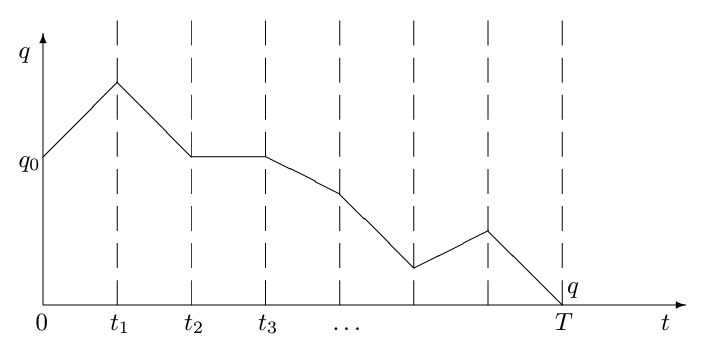
\includegraphics[width=11cm]{img/path_integral.png}
    \caption{経路積分の概要~\cite{osborn2014aqft}}\label{fig:path_integral}
  \end{center}
\end{figure}
\begin{equation}
  \begin{split}
    &K(t;x,x')
    =\braket{x|\exp\ab(-\frac{it}{\hbar}\hat{H})|x'}
    =\lim_{\substack{n\to\infty,\\t=\text{const.}}}
    \bra{x}
    \ab[
      \prod_{k=1}^n\exp\ab(-\frac{i}{\hbar}(t_k-t_{k-1})\hat{H})]
    \ket{x'} \\
    &=\lim_{\substack{n\to\infty,\\t=\text{const.}}}
    \bra{x}\exp\ab(-\frac{i}{\hbar}(t-t_{n-1})\hat{H})
    \ab[
      \prod_{k=1}^{n-1}
      \ab(\int\d x_k \ket{x_k}\bra{x_k})
      \exp\ab(-\frac{i}{\hbar}(t_{k}-t_{k-1})\hat{H})
    ]
    \ket{x'} \\
    &=\lim_{\substack{\Delta t\to0\\n\Delta t=t}}
    \int\ab(\prod_{k=1}^{n-1}\d x_k)
    \prod_{k=0}^{n-1}
    \ab[
      \braket{x_{k+1}|\exp\ab(-\frac{i}{\hbar}\Delta t\hat{H})|x_k}
    ]
  \end{split}
\end{equation}
ここで総乗で現れる因子を評価するために
次の形のハミルトニアン$\hat{H}$を考える。
\begin{equation}
  \hat{H}=\frac{1}{2m}\hat{p}^2+V(\hat{x})
\end{equation}
その上で次の Campbell-Baker-Hausdorff の公式を使う。
\begin{equation}
  \begin{split}
    &\exp(\epsilon\hat{A})\exp(\epsilon\hat{B})
    =\exp\ab(\epsilon\hat{A}+\epsilon\hat{B}
    +\frac{1}{2}\epsilon^2\ab[\hat{A},\hat{B}]
    +\mathcal{O}(\epsilon^3)) \\
    &\Rightarrow
    \lim_{\epsilon\to0}
    \exp(\epsilon\hat{A})\exp(\epsilon\hat{B})
    =\lim_{\epsilon\to0}
    \exp\ab(\epsilon\hat{A}+\epsilon\hat{B})
  \end{split}
\end{equation}
このとき因子は次のように評価できる。
\begin{equation}
  \begin{split}
    &\lim_{\substack{\Delta t\to0\\n\Delta t=t}}
    \braket{x_{k+1}|\exp\ab(-\frac{i}{\hbar}\Delta t\hat{H})|x_k}
    =\lim_{n\to\infty}
    \braket{x_{k+1}|\exp\ab(-\frac{i}{\hbar}\Delta t
      \ab(\frac{1}{2m}\hat{p}^2+V(\hat{x}))
      )|x_k}  \\
    &=\lim_{\substack{\Delta t\to0\\n\Delta t=t}}
    \braket{x_{k+1}|
      \exp\ab(-\frac{i}{\hbar}\Delta t
      \frac{1}{2m}\hat{p}^2)
      \exp\ab(-\frac{i}{\hbar}\Delta t
      V(\hat{x}))
      |x_k} \\
    &=\lim_{\substack{\Delta t\to0\\n\Delta t=t}}
    \exp\ab(-\frac{i}{\hbar}\Delta tV(x_k))
    \braket{x_{k+1}|
      \exp\ab(-\frac{i}{\hbar}\Delta t
      \frac{1}{2m}\hat{p}^2)
      |x_k}
  \end{split}
\end{equation}
運動量演算子$\hat{p}$に関する完全性関係を用いて次を得る。
\begin{equation}
  \begin{split}
    &\braket{x_{k+1}|
      \exp\ab(-\frac{i}{\hbar}\Delta t
      \frac{1}{2m}\hat{p}^2)
      |x_k}
    =\braket{x_{k+1}|
      \exp\ab(-\frac{i}{\hbar}\Delta t
      \frac{1}{2m}\hat{p}^2)
      \ab(\int\d p\ket{p}\bra{p})
      |x_k} \\
    &=\int\d p
    \exp\ab(-\frac{i}{\hbar}\Delta t
    \frac{1}{2m}p^2)
    \braket{x_{k+1}|p}
    \braket{p|x_{k}}
    \overset{(\ref{eq:xp_eigenfunction})}{=}
    \int\d p
    \exp\ab(-\frac{i}{\hbar}\Delta t
    \frac{1}{2m}p^2)
    \frac{1}{2\pi\hbar}e^{\frac{i}{\hbar}p(x_{k+1}-x_k)} \\
    &=\frac{1}{2\pi\hbar}\int_{-\infty}^\infty\d p
    \exp\ab[
      -\frac{i}{2m\hbar}\Delta t
      \ab(p-m\frac{n}{t}(x_{k+1}-x_k))^2
      +i\frac{m}{2\hbar}\Delta t(x_{k+1}-x_k)^2
    ] \\
    &=\frac{1}{2\pi\hbar}
    \exp\ab[i\frac{m}{2\hbar}\Delta t(x_{k+1}-x_k)^2]
    \int_{-\infty}^\infty\d p
    \exp\ab[
      -\frac{i}{2m\hbar}\Delta tp^2
    ] \\
    &=\frac{1}{2\pi\hbar}
    \exp\ab(i\frac{m}{2\hbar\Delta t}(x_{k+1}-x_k)^2)
    \sqrt{\frac{2m\hbar}{\Delta t}}
    \int_{-\infty}^\infty\d P
    e^{-iP^2}
  \end{split}
\end{equation}
ここでフレネル積分の結果を用いると次がわかる。
\begin{equation}
  \begin{split}
    &\int_{-\infty}^\infty\d Pe^{-iP^2}
    =\overline{\int_{-\infty}^\infty\d P e^{iP^2}}
    =\overline{\sqrt{\frac{\pi}{2}}(1+i)}
    =\sqrt{\frac{\pi}{2}}(1-i)
    =\sqrt{\pi}e^{-i\pi/4}
    =\sqrt{\pi e^{-i\pi/2}}
    =\sqrt{\frac{\pi}{i}}
  \end{split}
\end{equation}
これより次の結果を得る。
\begin{equation}
  \label{eq:free_propagator}
  \begin{split}
    &\braket{x_{k+1}|
      \exp\ab(-\frac{i}{\hbar}\Delta t
      \frac{1}{2m}\hat{p}^2)
      |x_k}
    =\sqrt{\frac{m}{2\pi i\hbar\Delta t}}
    \exp\ab(i\frac{m}{2\hbar\Delta t}(x_{k+1}-x_k)^2)
  \end{split}
\end{equation}
これは微小区間に対する伝搬関数であるが、
繰り返し適用することで有限の区間に対してもそのまま拡張できる。
したがって伝搬関数は次のように書ける。
\begin{equation}
  \begin{split}
    &K(t;x,x')
    =\lim_{\substack{\Delta t\to0\\n\Delta t=t}}
    \int\ab(\prod_{k=1}^{n-1}\d x_k)
    \prod_{k=0}^{n-1}
    \ab[
      \sqrt{\frac{m}{2\pi i\hbar\Delta t}}
      \exp\ab(i\frac{m}{2\hbar\Delta t}(x_{k+1}-x_k)^2
      -\frac{i}{\hbar}\Delta tV(x_k))
    ] \\
    &=\lim_{\substack{\Delta t\to0\\n\Delta t=t}}
    \int\ab(
    \sqrt{\frac{m}{2\pi i\hbar\Delta t}}
    \prod_{k=1}^{n-1}\sqrt{\frac{m}{2\pi i\hbar\Delta t}}\d x_k) \\
    &\qquad\times\exp\ab(
    \sum_{k=0}^{n-1}
    \frac{i}{\hbar}\ab(
    \frac{m}{2}\ab(\frac{x_{k+1}-x_k}{\Delta t})^2-V(x_k)
    )\Delta t
    )
  \end{split}
\end{equation}
極限操作後の結果を次の形で書いて、この計算方法を経路積分と呼ぶ。
\begin{equation}
  \begin{split}
    &K(t;x,x')=\braket{x|\exp\ab(-\frac{it}{\hbar}\hat{H})|x'}
    =\int\d[x]\exp\ab(\frac{i}{\hbar}S[x]) \\
    &\d[x]\equiv
    \lim_{\substack{\Delta t\to0\\n\Delta t=t}}
    \sqrt{\frac{m}{2\pi i\hbar\Delta t}}
    \prod_{k=1}^{n-1}\sqrt{\frac{m}{2\pi i\hbar\Delta t}}\d x_k, \\
    &S[x]\equiv
    \lim_{\substack{\Delta t\to0\\n\Delta t=t}}
    \sum_{k=0}^{n-1}
    \ab(
    \frac{m}{2}\ab(\frac{x_{k+1}-x_k}{\Delta t})^2-V(x_k)
    )\Delta t
    =\int_0^t\d t'\ab(\frac{m}{2}\dot{x}^2-V(x))
    =\int_0^t\d t'L(x,\dot{x})
  \end{split}
\end{equation}
経路積分を用いることで古典的な作用から
量子的な伝搬関数を求めることができる。
経路積分は名前の通り始点から終点に至るすべてのケースを足し上げる。
足し上げの対象は古典的な作用を回転角とする位相因子である。

古典的な運動では作用原理$\delta S=0$が成立する経路を選択するが、
鞍点近似法からこれは経路積分のうち最も寄与の大きい経路になる。
つまり位相がゆるやかに振動する経路は積分値が大きくなるが、
位相が高速振動する経路は各地点の値が打ち消しあって積分値が小さくなる。
このような古典論に基づく運動の条件を on-shell 条件と呼ぶ。
経路積分では on-shell 条件を満たす経路が主要項となる。
経路積分では古典的な経路を主とし、
量子効果で可能となる経路を補正として加えて計算する。

\subsubsection{調和振動子の伝搬関数の導出}

調和振動子の作用に対して経路積分を計算することで伝搬関数を求める。
前述の通り主要項は on-shell 条件を満たすので、
経路を古典論における解とそこからの差分で表現する。
まずは古典論における調和振動子の解を求める。
古典的な調和振動子のハミルトニアンは次の通りである。
\begin{equation}
  H=\frac{1}{2m}p^2+\frac{m\omega^2}{2}x^2
\end{equation}
ハミルトニアンが与えられる場合、
古典論における運動方程式は正準方程式で与えられる。
\begin{equation}
  \begin{split}
    &\dot{x}=\pdv{H}{p}=\frac{p}{m},\quad
    \dot{p}=-\pdv{H}{q}=-m\omega^2 x \\
    &\Rightarrow
    \ddot{x}=-\omega^2 x
  \end{split}
\end{equation}
この運動方程式が on-shell 条件である。
この方程式を境界条件$x(0)=x',x(t)=x$と合わせて解く。
この解$\bar{x}(t')$は次の通り。
\begin{equation}
  \begin{split}
    &\bar{x}(t')=A\sin(\omega t')+B\cos(\omega t')
    \Rightarrow
    \begin{cases}
      x'=B \\
      x=A\sin(\omega t)+B\cos(\omega t)
    \end{cases}
    \Rightarrow
    A=\frac{x-x'\cos(\omega t)}{\sin(\omega t)} \\
    &\Rightarrow
    \bar{x}(t')=\frac{x-x'\cos(\omega t)}{\sin(\omega t)}\sin(\omega t')+x'\cos(\omega' t)
    =\frac{1}{\sin(\omega t)}\ab[
      \sin(\omega t')x+\sin(\omega(t-t'))x'
    ]
  \end{split}
\end{equation}
この解$\bar{x}(t')$を作用$S[x]$に代入することで
on-shell 条件を課した際の作用である on-shell 作用が求まる。
\begin{equation}
  \begin{split}
    S[\bar{x}]
    &=\frac{m}{2}\int_0^t\d t'\ab(\dot{\bar{x}}(t')^2-\omega^2\bar{x}(t')^2)
    =\frac{m}{2}\ab[\bar{x}(t')\dot{\bar{x}}(t')]_{t'=0}^{t'=t}
    -\frac{m}{2}\int_0^t\d t'\bar{x}(t')(\ddot{\bar{x}}(t')+\omega^2\bar{x}(t')) \\
    &=\frac{m}{2}\ab(x\dot{\bar{x}}(t)-x'\dot{\bar{x}}(0))
    =\frac{m}{2}\ab(
    \frac{x}{\sin(\omega t)}\ab(
      \omega\cos(\omega t)x-\omega x')
    -\frac{x'}{\sin(\omega t)}\ab(
      \omega x-\omega\cos(\omega t) x')
    ) \\
    &=\frac{m\omega}{2}\frac{
      (x^2+x'^2)\cos(\omega t)-2xx'
    }{\sin(\omega t)}
  \end{split}
\end{equation}
作用(汎関数)を on-shell 作用の周りで展開する。
ただし時間軸の端点で境界条件を満たすように次の展開を考える。
\begin{equation}
  x(t')=\bar{x}(t')+\delta x(t'),\quad
  \delta x(0)=\delta x(t)=0
\end{equation}
このとき作用は on-shell 作用と$\delta x(t')$に関する作用で分離できる。
\begin{equation}
  \begin{split}
    &S[x]=S[\bar{x}+\delta x]
    =\int_0^t\d t'\ab(
    \frac{m}{2}\ab(\dot{\bar{x}}+\delta\dot{x})^2
    -\frac{1}{2}m\omega^2\ab(\bar{x}+\delta x)^2
    ) \\
    &=
    [\dot{\bar{x}}\delta x]_{t'=0}^{t'=t}+
    \frac{m}{2}\int_0^t\d t'\ab[
      (\dot{\bar{x}}^2-\omega^2\bar{x}^2)
      -2(\ddot{\bar{x}}+\omega^2\bar{x})\delta x
      +(\delta\dot{x}^2-\omega^2(\delta x)^2)
    ] \\
    &=\int_0^t\d t'
    \ab(\frac{m}{2}\dot{\bar{x}}^2-\frac{1}{2}m\omega^2\bar{x}^2)
    +\frac{m}{2}\int_0^t\d t'
    \ab(\frac{m}{2}\delta\dot{x}^2-\frac{1}{2}m\omega^2(\delta x)^2) \\
    &=S[\bar{x}]+S[\delta x]
  \end{split}
\end{equation}
積分測度については次が成立する。
\begin{equation}
  \d[x]=\d[\bar{x}+\delta x]=\d[\delta x]
\end{equation}

よって鞍点評価で経路積分は次の形に帰着する。
\begin{equation}
  K(t;x,x')
  =\int\d[x]\exp\ab(\frac{i}{\hbar}S[x])
  =\exp\ab(\frac{i}{\hbar}S[\bar{x}])
  \int\d[\delta x]\exp\ab(\frac{i}{\hbar}S[\delta x])
\end{equation}
よって$\delta x$に関する経路積分を評価すればよい。
$\delta x(t')$は積分区間の端点で0になるので、
これに基づきフーリエ級数展開ができる。
$n,m\in\mathbb{Z}_+$として次の直交関係を用いる。
\begin{equation}
  \begin{split}
    &\int_0^t\d t'\ab(\sin\frac{n\pi t'}{t})\ab(\sin\frac{m\pi t'}{t})
    =\int_0^t\d t'
    \frac{e^{i\frac{n\pi t'}{t}}-e^{-i\frac{n\pi t'}{t}}}{2i}
    \frac{e^{i\frac{m\pi t'}{t}}-e^{-i\frac{m\pi t'}{t}}}{2i} \\
    &=\frac{1}{2}\int_0^t\d t'
    \ab(
    \frac{e^{i\frac{(n-m)\pi t'}{t}}+e^{-i\frac{(n-m)\pi t'}{t}}}{2}
    -\frac{e^{i\frac{(n+m)\pi t'}{t}}+e^{-i\frac{(n+m)\pi t'}{t}}}{2}
    ) \\
    &=\frac{1}{2}\int_0^t\d t'
    \ab(
    \cos\ab((n-m)\frac{\pi t'}{t})
    -\cos\ab((n+m)\frac{\pi t'}{t})
    )
  \end{split}
\end{equation}
ここで$n=m$であれば次が成立。
\begin{equation}
  \begin{split}
    &\int_0^t\d t'\ab(\sin\frac{n\pi t'}{t})\ab(\sin\frac{n\pi t'}{t})
    =\frac{1}{2}\int_0^t\d t'\ab(1-\cos\frac{2n\pi t'}{t}) \\
    &=\frac{1}{2}\ab[t'-\frac{t}{2n\pi}\sin\frac{2n\pi t'}{t}]_{t'=0}^{t'=t}
    =\frac{t}{2}
  \end{split}
\end{equation}
$n\neq m$であれば次が成立。
\begin{equation}
  \begin{split}
    &\int_0^t\d t'\ab(\sin\frac{n\pi t'}{t})\ab(\sin\frac{m\pi t'}{t}) \\
    &=\frac{1}{2}\ab[
      \frac{t}{(n-m)\pi}\sin\ab((n-m)\frac{\pi t'}{t})
      -\frac{t}{(n+m)\pi}\sin\ab((n+m)\frac{\pi t'}{t})
    ]_{t'=0}^{t'=t} \\
    &=0
  \end{split}
\end{equation}
よって規格化条件も含めて次で展開できる。
\begin{equation}
  \delta x(t')
  =\sqrt{\frac{2}{t}}\sum_{n=1}^\infty
  a_n \sin\frac{n\pi t'}{t}
\end{equation}
ここで$\delta x(t')$の関数自由度は係数$a_n$の自由度に帰着することに気を付ける。

この展開を用いると古典的な作用は次のように書ける。
\begin{equation}
  \begin{split}
    &S[\delta x]
    =\frac{m}{2}\int_0^t\d t'
    \ab(\frac{m}{2}\delta\dot{x}^2-\frac{1}{2}m\omega^2(\delta x)^2)
    =\ab[\frac{m}{2}\delta\dot{x}\delta x]_{t'=0}^{t'=t}
    -\frac{m}{2}\int_0^t\d t'
    \delta x\ab(\delta\ddot{x}+\omega^2\delta x) \\
    &=-\frac{m}{2}\int_0^t\d t'
    \ab(\sqrt{\frac{2}{t}}\sum_{n=1}^\infty
    a_n \sin\frac{n\pi t'}{t})
    \ab(\sqrt{\frac{2}{t}}\sum_{k=1}^\infty
    \ab(\omega^2-\frac{k^2\pi^2}{t^2})
    a_k \sin\frac{k\pi t'}{t}) \\
    &=\frac{m}{t}\sum_{n=1}^\infty\sum_{k=1}^\infty
    a_n a_k
    \ab(\frac{k^2\pi^2}{t^2}-\omega^2)
    \int_0^t\d t'
    \sin\frac{n\pi t'}{t}
    \sin\frac{k\pi t'}{t} \\
    &=\frac{m}{t}\sum_{n=1}^\infty\sum_{k=1}^\infty
    a_n a_k
    \ab(\frac{k^2\pi^2}{t^2}-\omega^2)
    \frac{t}{2}\delta_{n,k}
    =\frac{m}{2}\sum_{n=1}^\infty
    a_n^2
    \ab(\frac{n^2\pi^2}{t^2}-\omega^2)
  \end{split}
\end{equation}
ただし被積分関数が一様収束することから
積分と無限級数を入れ替えた。

積分測度は$\delta x$の関数自由度に対して定義される。
これはフーリエ級数展開を用いると$a_n$の自由度に帰着される。
そこで$\delta x$が$a_n$について線形であることを用いて、
ある規格化因子$C$を使って次のように書く。
\begin{equation}
  \d[\delta x]
  =C\prod_{n=1}^\infty\d a_n
\end{equation}

これらをまとめると$\delta x$に対する経路積分は次のように書ける。
\begin{equation}
  \begin{split}
    &\int\d[\delta x]e^{iS[\delta x]}
    =C\prod_{n=1}^\infty\int\d a_n
    \exp\ab(\frac{i}{\hbar}\frac{m}{2}a_n^2\ab(\frac{n^2\pi^2}{t^2}-\omega^2)) \\
    &=C\prod_{n=1}^\infty
    \frac{1}{\sqrt{\frac{m}{2\hbar}\ab(\frac{n^2\pi^2}{t^2}-\omega^2)}}
    \int\d a_n e^{ia_n^2}
    =C\prod_{n=1}^\infty
    \sqrt{\frac{\pi i}{\frac{m}{2\hbar}\ab(\frac{n^2\pi^2}{t^2}-\omega^2)}}
  \end{split}
\end{equation}
ここでフレネル積分を適用した。
いま自由粒子のケース$\omega=0$を考え、
(\ref{eq:free_propagator})を適用することで
規格化因子$C$が次を満たすことがわかる。
\begin{equation}
  \begin{split}
    &K(t;x,x')
    =\exp\ab(\frac{i}{\hbar}S[\bar{x}])
    \int\d[\delta x]\exp\ab(\frac{i}{\hbar}S[\delta x]) \\
    &=\exp\ab(\frac{i}{\hbar}
    \frac{m\omega}{2}\frac{
        (x^2+x'^2)\cos(\omega t)-2xx'
      }{\sin(\omega t)})
    \int\d[\delta x]\exp\ab(\frac{i}{\hbar}S[\delta x]) \\
    &\Rightarrow
    \sqrt{\frac{m}{2\pi i\hbar t}}
    \exp\ab(i\frac{m}{2\hbar t}(x-x')^2)
    =\exp\ab(i
    \frac{m}{2\hbar t}(x-x')^2)
    C\prod_{n=1}^\infty
    \sqrt{\frac{\pi i}{\frac{m}{2\hbar}\frac{n^2\pi^2}{t^2}}} \\
    &\Rightarrow
    \sqrt{\frac{m}{2\pi i\hbar t}}
    =C\prod_{n=1}^\infty
    \sqrt{\frac{\pi i}{\frac{m}{2\hbar}\frac{n^2\pi^2}{t^2}}} \\
  \end{split}
\end{equation}
よってこれを用いて経路積分は次のように書ける。
\begin{equation}
  \begin{split}
    &\int\d[\delta x]e^{iS[\delta x]}
    =\sqrt{\frac{m}{2\pi i\hbar t}}
    \prod_{n=1}^\infty
    \frac{1}{\sqrt{1-\ab(\frac{\omega t}{n\pi})^2}}
  \end{split}
\end{equation}
ここで次の三角関数の無限累積展開を用いる。
\begin{equation}
  \sin(x)
  =x\prod_{n=1}^\infty\ab(1-\frac{x}{n\pi})\ab(1+\frac{x}{n\pi})
\end{equation}
この公式はワイエルシュトラスの因数分解定理などから確かめられる。
直感的には$\sin(x)$が$x=n\pi,\,n\in\mathbb{Z}$で0となることからわかる。
これにより次を得る。
\begin{equation}
  \begin{split}
    &\int\d[\delta x]e^{iS[\delta x]}
    =\sqrt{\frac{m}{2\pi i\hbar t}}
    \sqrt{
      \frac{\omega t}{\sin(\omega t)}
    }
    =\sqrt{\frac{m\omega}{2\pi i\hbar\sin(\omega t)}}
  \end{split}
\end{equation}
したがって調和振動子の伝搬関数として次を得る。
\begin{equation}
  \begin{split}
    &K(t;x,x')
    =\exp\ab(\frac{i}{\hbar}S[\bar{x}])
    \int\d[\delta x]\exp\ab(\frac{i}{\hbar}S[\delta x]) \\
    &=\sqrt{\frac{m\omega}{2\pi i\hbar\sin(\omega t)}}
    \exp\ab(\frac{i}{\hbar}
    \frac{m\omega}{2}\frac{
        (x^2+x'^2)\cos(\omega t)-2xx'
      }{\sin(\omega t)})
  \end{split}
\end{equation}